% Présentation (15 min) – Station de sécurité Raspberry Pi
% Compilation : xelatex presentation.tex (deux fois)
\documentclass[aspectratio=169,11pt]{beamer}
\usetheme[progressbar=frametitle, numbering=fraction]{metropolis}
\usepackage{fontspec}
\setsansfont{Noto Sans}
\setmonofont{Noto Sans Mono}[Scale=0.85]
\usepackage[french]{babel}
\usepackage{booktabs,tabularx,tikz,listings}
\usetikzlibrary{positioning,arrows.meta,calc}
\graphicspath{{figures/captures/}{figures/wireframes/}}

\definecolor{accent}{HTML}{1D6FB8}
\definecolor{ok}{HTML}{1E8A4C}
\definecolor{partiel}{HTML}{B7791F}
\definecolor{non}{HTML}{C0392B}
\setbeamercolor{frametitle}{bg=accent!85!black}
\setbeamercolor{progress bar}{fg=accent}
\setbeamercolor{alerted text}{fg=non}

\lstset{language=Python, basicstyle=\ttfamily\scriptsize, keywordstyle=\color{accent}\bfseries,
  commentstyle=\color{gray}, stringstyle=\color{ok}, showstringspaces=false, frame=single,
  rulecolor=\color{black!15}, backgroundcolor=\color{black!3}}
\newcommand{\src}[1]{../../security_station/#1}

\title{Station de sécurité Raspberry Pi}
\subtitle{Projet intégré : système de contrôle-commande Dual-UI}
\author{Marc Robison}
\institute{INSA Hauts-de-France -- 5A ESE -- Prototypage des systèmes embarqués\\Enseignant : M. Alain Allouis}
\date{17 novembre 2026}

\begin{document}

\maketitle

% ---------------------------------------------------------------------------
\begin{frame}{Le projet en bref}
\begin{columns}[T]
\column{0.42\textwidth}
Surveiller une pièce et donner l'alerte.
\medskip
\begin{itemize}
  \item \textbf{3 capteurs} simulés : ultrason, PIR, DHT22
  \item \textbf{2 actionneurs} : relais, buzzer
  \item \textbf{2 interfaces} en même temps : Qt sur la Pi, web sur PC ou téléphone
\end{itemize}
\column{0.56\textwidth}
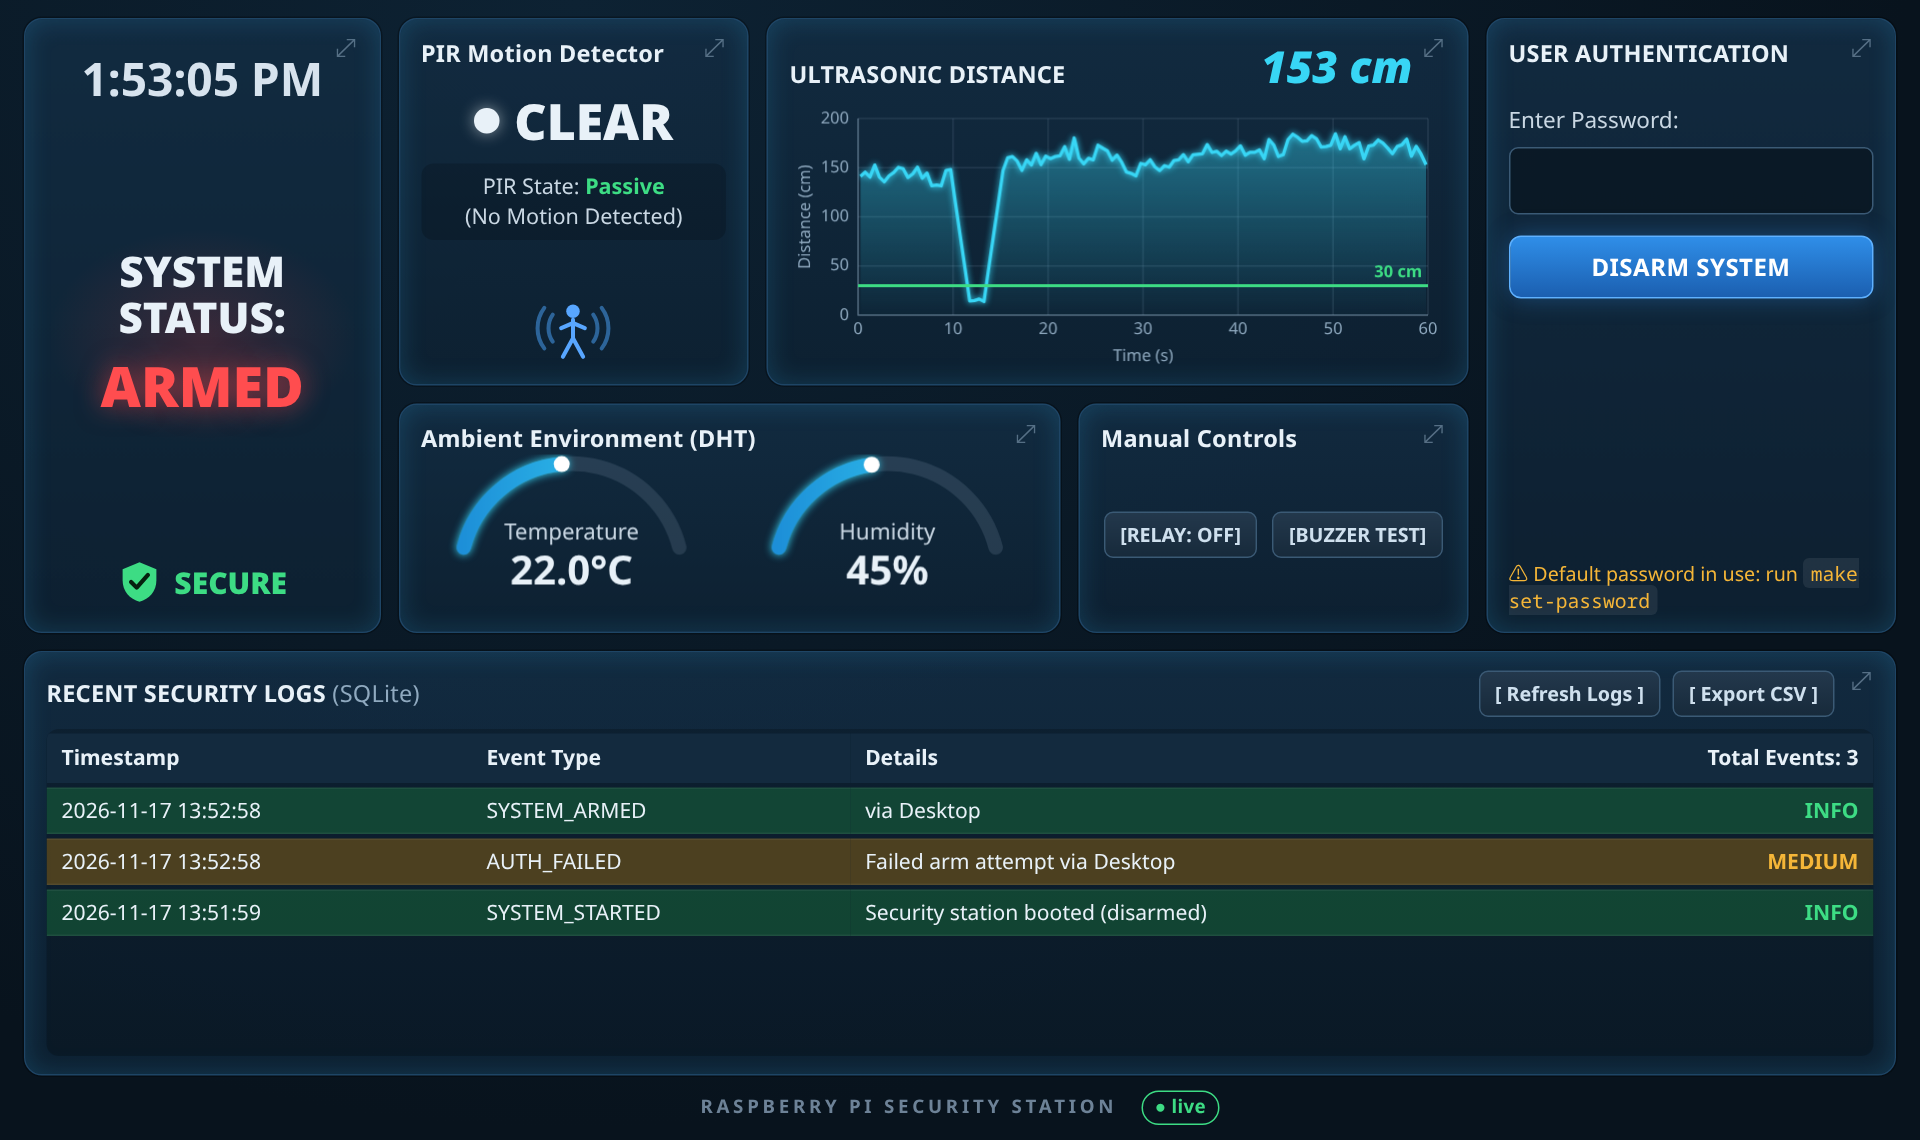
\includegraphics[width=\linewidth]{web_2_normal.png}
\end{columns}
\end{frame}

% ---------------------------------------------------------------------------
\begin{frame}{Parcours utilisateur et maquette}
\begin{columns}[c]
\column{0.6\textwidth}
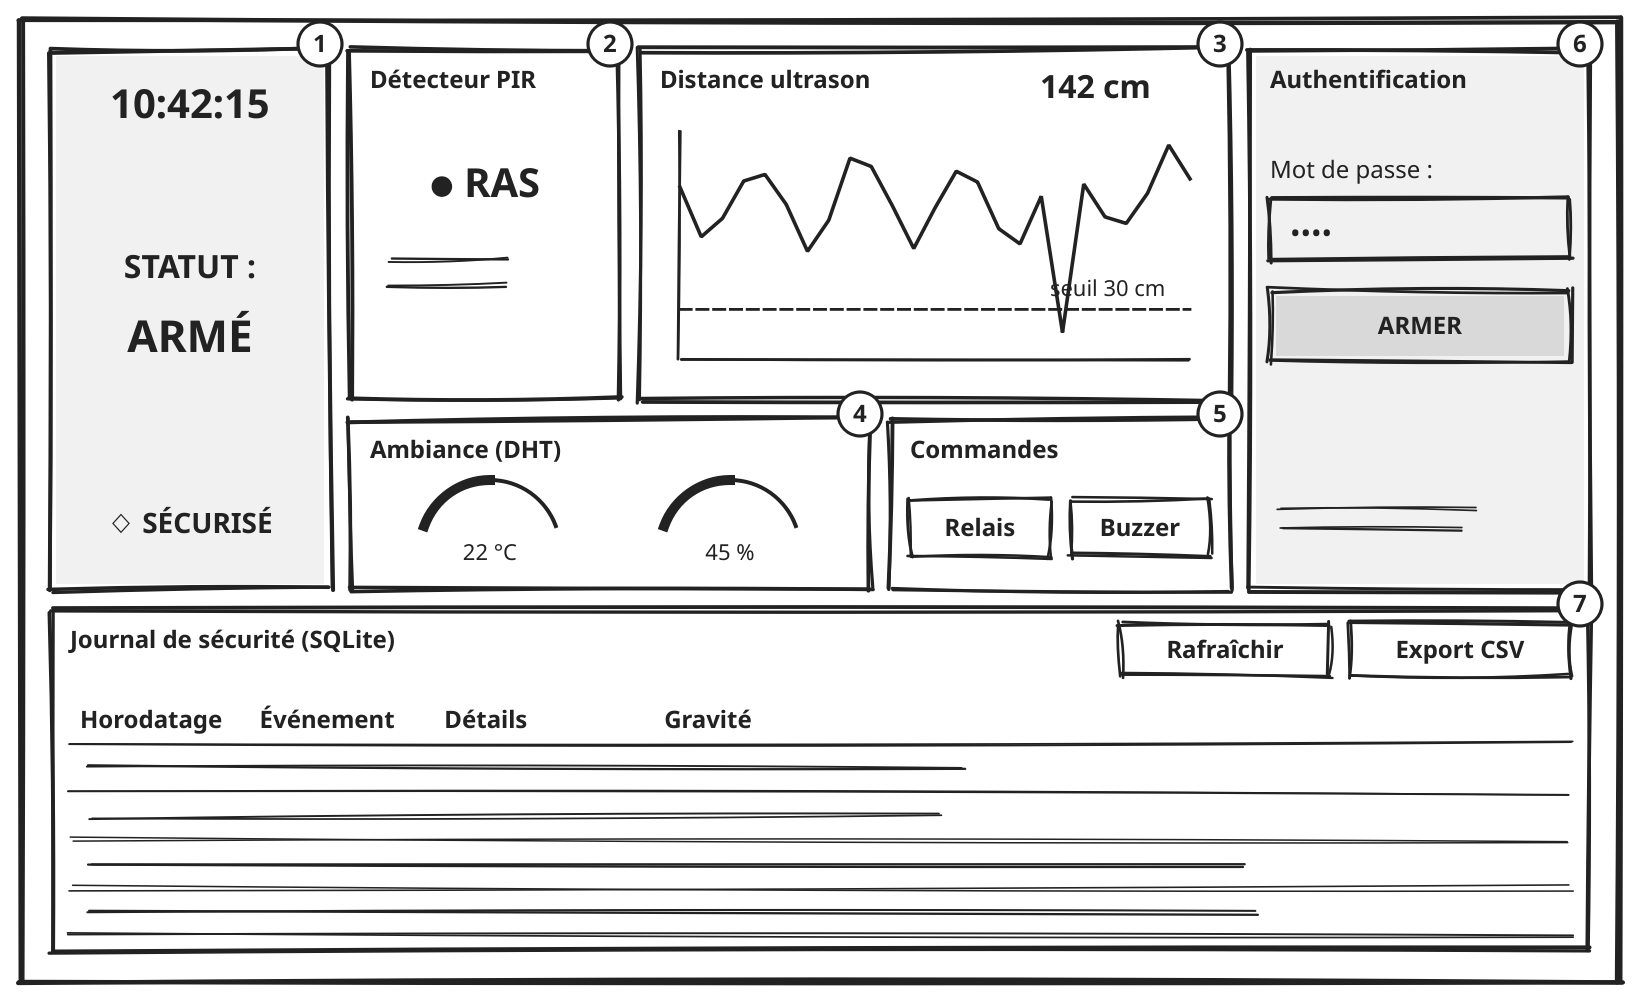
\includegraphics[width=\linewidth]{wf_principal.png}
\column{0.38\textwidth}
Trois parcours :
\begin{enumerate}
  \item \textbf{Regarder} : cliquer une tuile $\rightarrow$ vue agrandie $\rightarrow$ retour
  \item \textbf{Agir} : mot de passe $\rightarrow$ armer / désarmer
  \item \textbf{Être alerté} : alarme $\rightarrow$ ALERT + buzzer + journal
\end{enumerate}
\medskip
Même organisation sur Qt et sur le web.
\end{columns}
\end{frame}

% ---------------------------------------------------------------------------
\begin{frame}{Micro-interaction : l'alarme d'intrusion}
\small
\begin{tabular}{>{\bfseries}p{2.7cm} p{10.6cm}}
\toprule
Déclencheur & Le système voit un objet à moins de 30~cm, ou un mouvement, \alert{alors que la station est armée}. \\
Règles & Comparer au seuil $\rightarrow$ enregistrer l'événement (SQLite, horodaté) $\rightarrow$ statut ALERT. \\
Retour & « ALERT » rouge qui clignote, valeur en rouge, ligne dans le journal, buzzer. Pareil sur le web en moins d'1~s. \\
Boucles et modes & Seulement en mode armé. L'alerte reste 5~s. Pas de nouvelle alerte tant que la distance ne repasse pas au-dessus de 40~cm. \\
\bottomrule
\end{tabular}
\bigskip

Deux autres micro-interactions sont détaillées dans le rapport : \textbf{armer / désarmer} et \textbf{commander un actionneur}.
\end{frame}

% ---------------------------------------------------------------------------
\begin{frame}{Architecture : une seule Station}
\centering
\resizebox{0.95\linewidth}{!}{%
\begin{tikzpicture}[
  font=\small,
  b/.style={draw, rounded corners=3pt, align=center, minimum width=2.7cm, minimum height=10mm, fill=white},
  c/.style={b, fill=accent!15, minimum width=2.9cm, minimum height=14mm},
  arr/.style={-{Stealth[length=2mm]}, thick},
  two/.style={{Stealth[length=2mm]}-{Stealth[length=2mm]}, thick}]
  \node[c] (st) at (0,0) {\textbf{Station}\\(station.py)};
  \node[b] (sim) at (-4.4,0) {Simulateur};
  \node[b] (db)  at (0,2.1) {SQLite};
  \node[b] (qt)  at (4.6,1.5) {Interface Qt};
  \node[b] (srv) at (4.6,-1.5) {Serveur HTTPS};
  \node[b] (nav) at (8.9,-1.5) {Navigateur};
  \draw[arr] (sim) -- node[above, font=\scriptsize]{mesures} (st);
  \draw[two] (st) -- node[right, font=\scriptsize]{événements} (db);
  \draw[two] (st.east) ++(0,0.3) -- node[above, sloped, font=\scriptsize]{signaux Qt} (qt.west);
  \draw[two] (st.east) ++(0,-0.3) -- node[below, sloped, font=\scriptsize]{état / actions} (srv.west);
  \draw[arr] ([yshift=2mm]srv.east) -- node[above, font=\scriptsize]{SSE} ([yshift=2mm]nav.west);
  \draw[arr] ([yshift=-2mm]nav.west) -- node[below, font=\scriptsize]{POST} ([yshift=-2mm]srv.east);
\end{tikzpicture}}
\bigskip

Tout part de la Station $\Rightarrow$ Qt et le web affichent toujours la même chose.
\end{frame}

% ---------------------------------------------------------------------------
\begin{frame}[fragile]{Simulation des capteurs}
\begin{columns}[T]
\column{0.4\textwidth}
\small
\begin{itemize}
  \item Ultrason : environ 160~cm, parfois une « approche » sous 30~cm
  \item PIR : un mouvement toutes les 20 à 90~s
  \item DHT22 : 19--25~°C, 35--60~\%
\end{itemize}
\medskip
Le simulateur appelle seulement \texttt{station.update\_...()}.\\[0.3em]
$\Rightarrow$ De vrais capteurs pourraient le remplacer sans toucher aux interfaces.
\column{0.58\textwidth}
\lstinputlisting[firstline=100,lastline=116,numbers=none,basicstyle=\ttfamily\tiny]{\src{simulator.py}}
\end{columns}
\end{frame}

% ---------------------------------------------------------------------------
\begin{frame}{Base de données et sécurité}
\begin{columns}[T]
\column{0.48\textwidth}
\textbf{SQLite}
\begin{itemize}
  \item Table \texttt{events} : horodatage, type, détails, gravité
  \item On garde les 1000 derniers événements
  \item Export CSV (Qt et web)
  \item Table \texttt{settings} : l'état armé survit à un redémarrage
\end{itemize}
\column{0.48\textwidth}
\textbf{Sécurité}
\begin{itemize}
  \item Mot de passe pour \emph{chaque} action
  \item Stocké en empreinte \emph{scrypt}, jamais en clair
  \item Échecs enregistrés (AUTH\_FAILED + origine)
  \item Web en HTTPS : rien ne passe en clair sur le Wi-Fi
\end{itemize}
\end{columns}
\end{frame}

% ---------------------------------------------------------------------------
\begin{frame}{Temps réel entre Qt et le web}
\begin{itemize}
  \item Le serveur web tourne dans un \textbf{thread à part} : l'écran Qt ne bloque jamais.
  \item \textbf{Station $\rightarrow$ navigateur} : Server-Sent Events, environ 2 mises à jour par seconde.
  \item \textbf{Navigateur $\rightarrow$ Station} : \texttt{POST /api/action} avec le mot de passe.
  \item Une action web est exécutée sur le \textbf{thread Qt}, pour éviter les conflits.
  \item Si la connexion tombe, le navigateur se reconnecte tout seul.
\end{itemize}
\bigskip
\small\textcolor{partiel}{Écart :} le sujet demande des WebSockets (FastAPI / Tornado). \texttt{QtHttpServer} a été essayé, mais il ne
renvoie que du texte. J'ai donc utilisé le serveur standard de Python avec SSE.
\end{frame}

% ---------------------------------------------------------------------------
\begin{frame}{Démo : lecture normale}
\centering
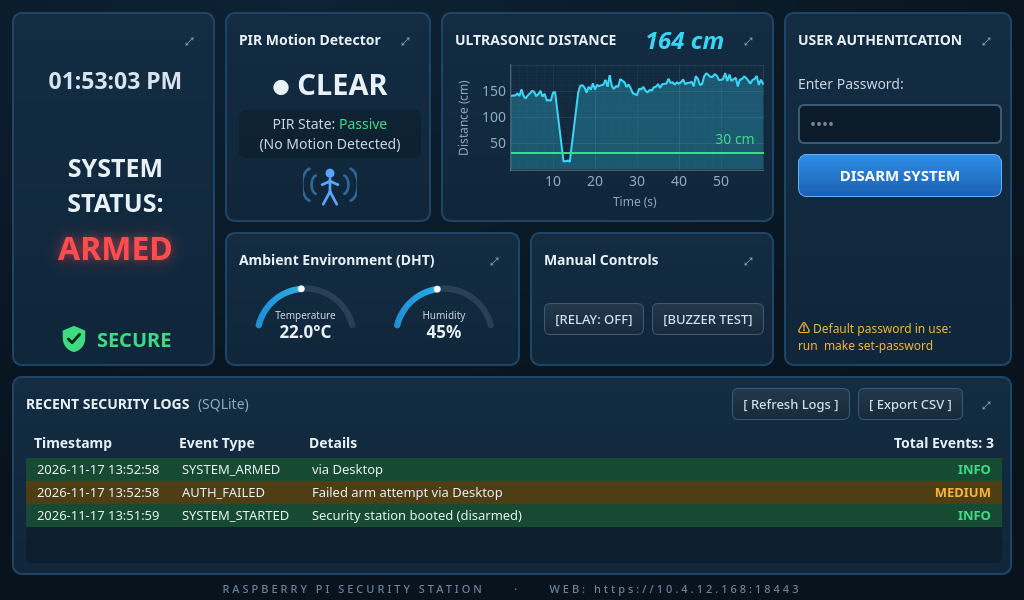
\includegraphics[width=0.49\linewidth]{qt_2_normal.png}\hfill
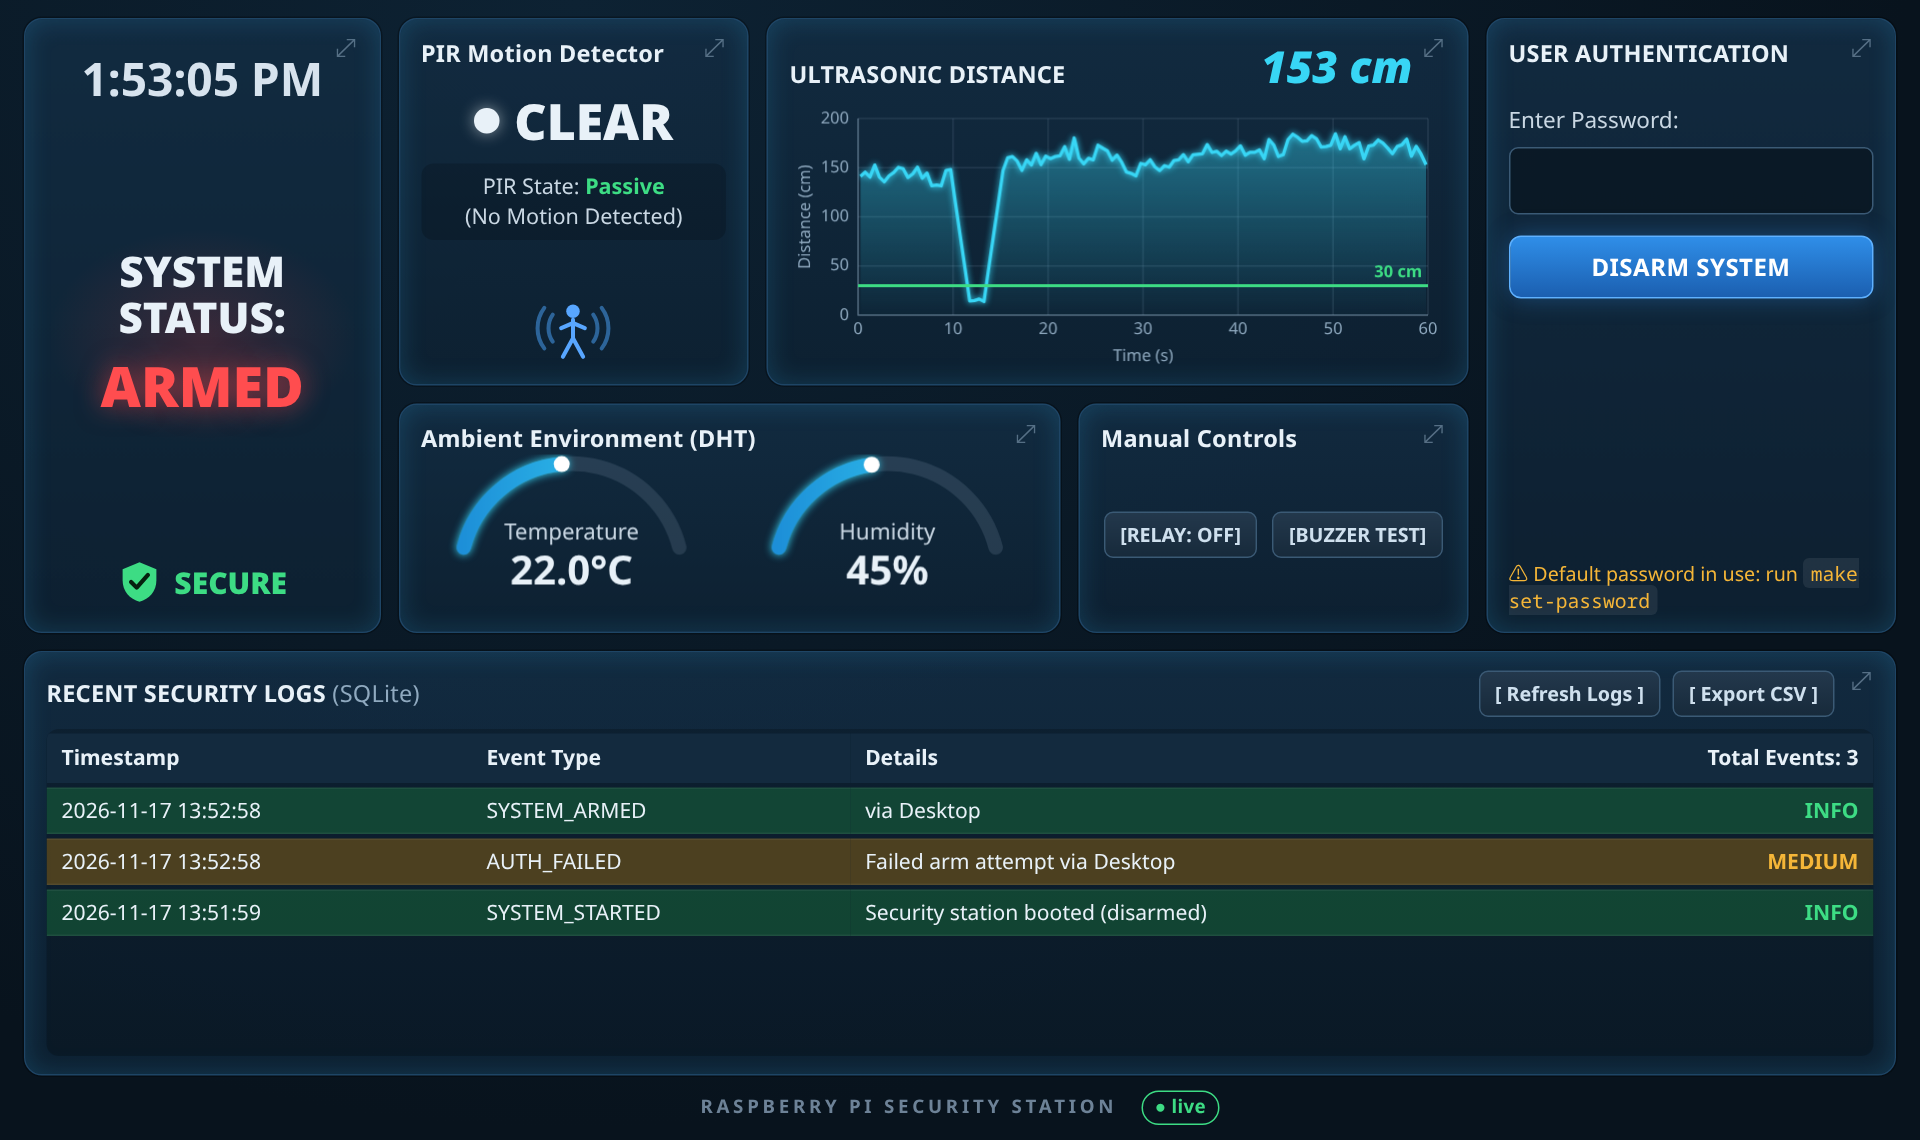
\includegraphics[width=0.49\linewidth]{web_2_normal.png}\\[0.5em]
\small Armée, sans menace : statut « SECURE ». À gauche Qt, à droite le web.
\end{frame}

% ---------------------------------------------------------------------------
\begin{frame}{Démo : alarme (seuil dépassé)}
\centering
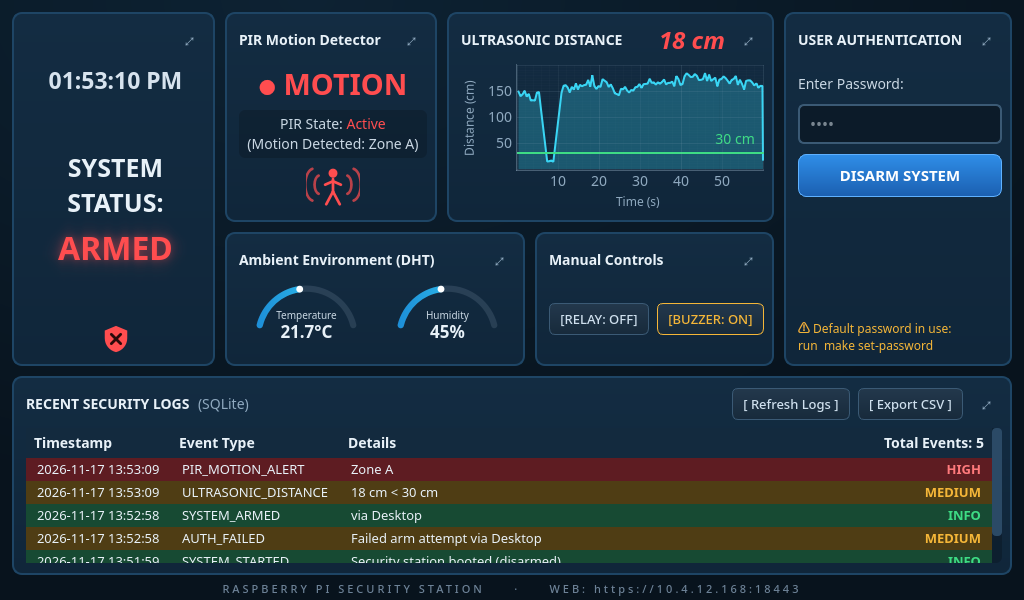
\includegraphics[width=0.49\linewidth]{qt_3_alarme.png}\hfill
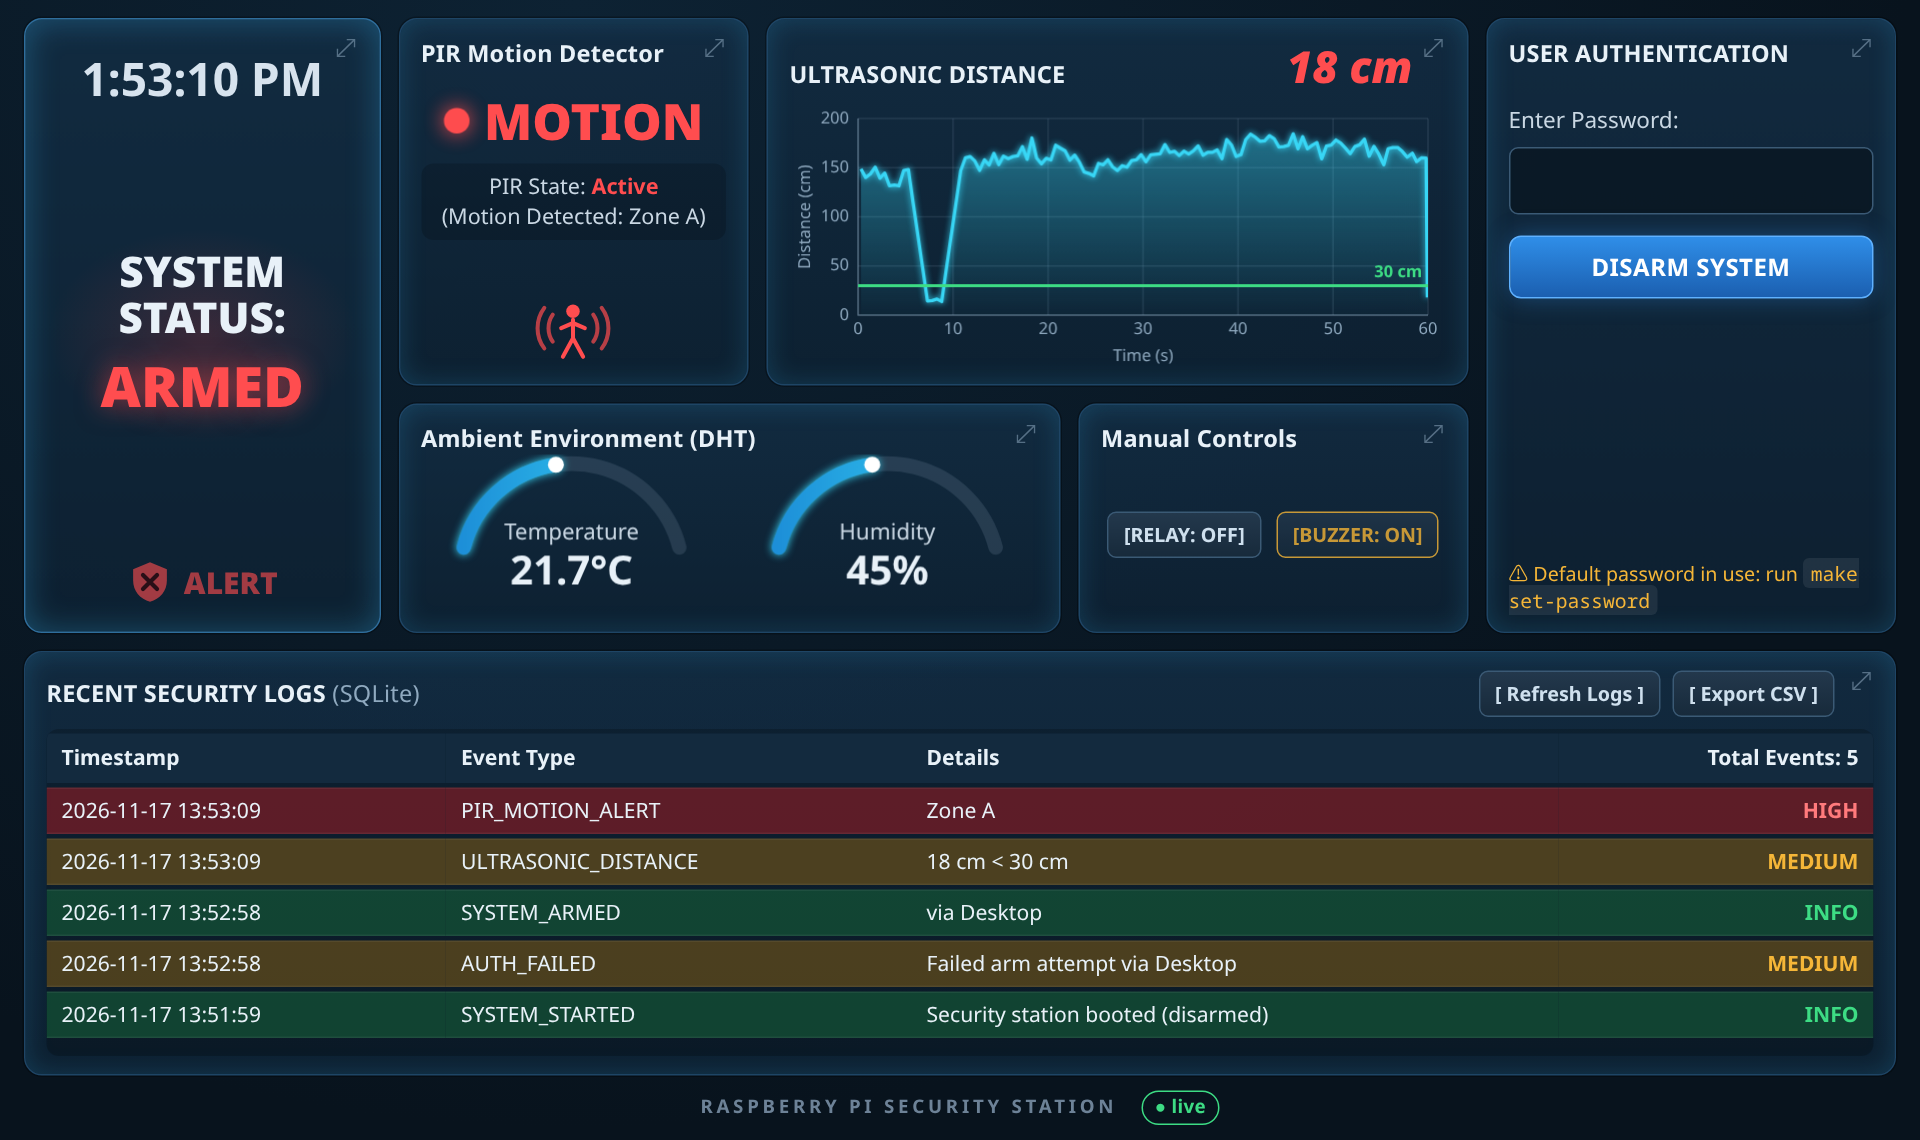
\includegraphics[width=0.49\linewidth]{web_3_alarme.png}\\[0.5em]
\small Objet à 18~cm + mouvement : tout passe au rouge, buzzer actif, 2 lignes d'alarme dans le journal.
\end{frame}

% ---------------------------------------------------------------------------
\begin{frame}{Démo : téléphone, déconnexion, vue agrandie}
\centering
\begin{minipage}[c]{0.15\linewidth}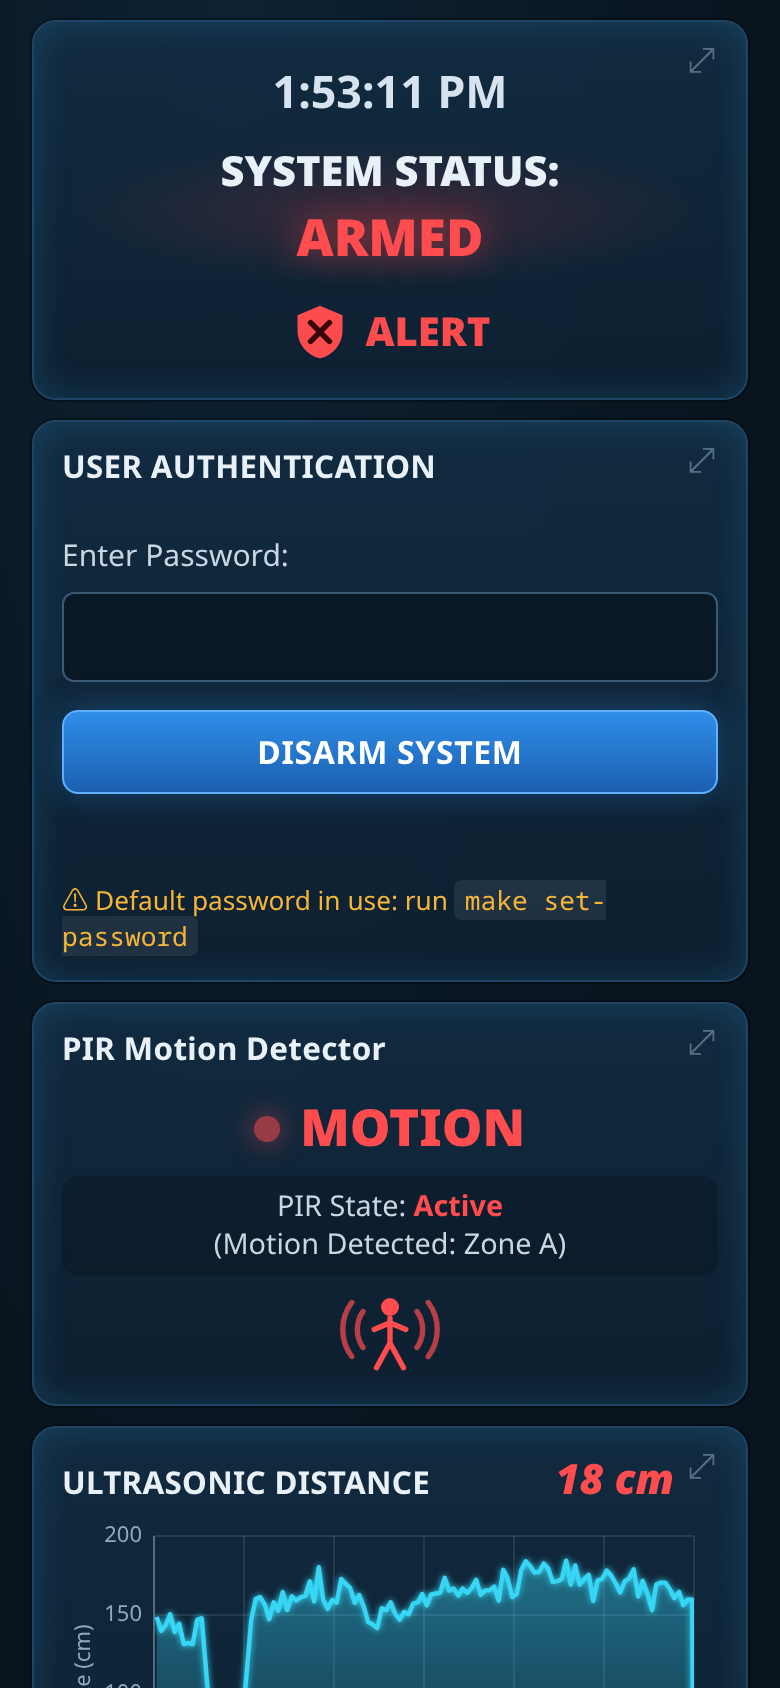
\includegraphics[width=\linewidth]{mobile_3_alarme.png}\end{minipage}\hspace{2mm}
\begin{minipage}[c]{0.15\linewidth}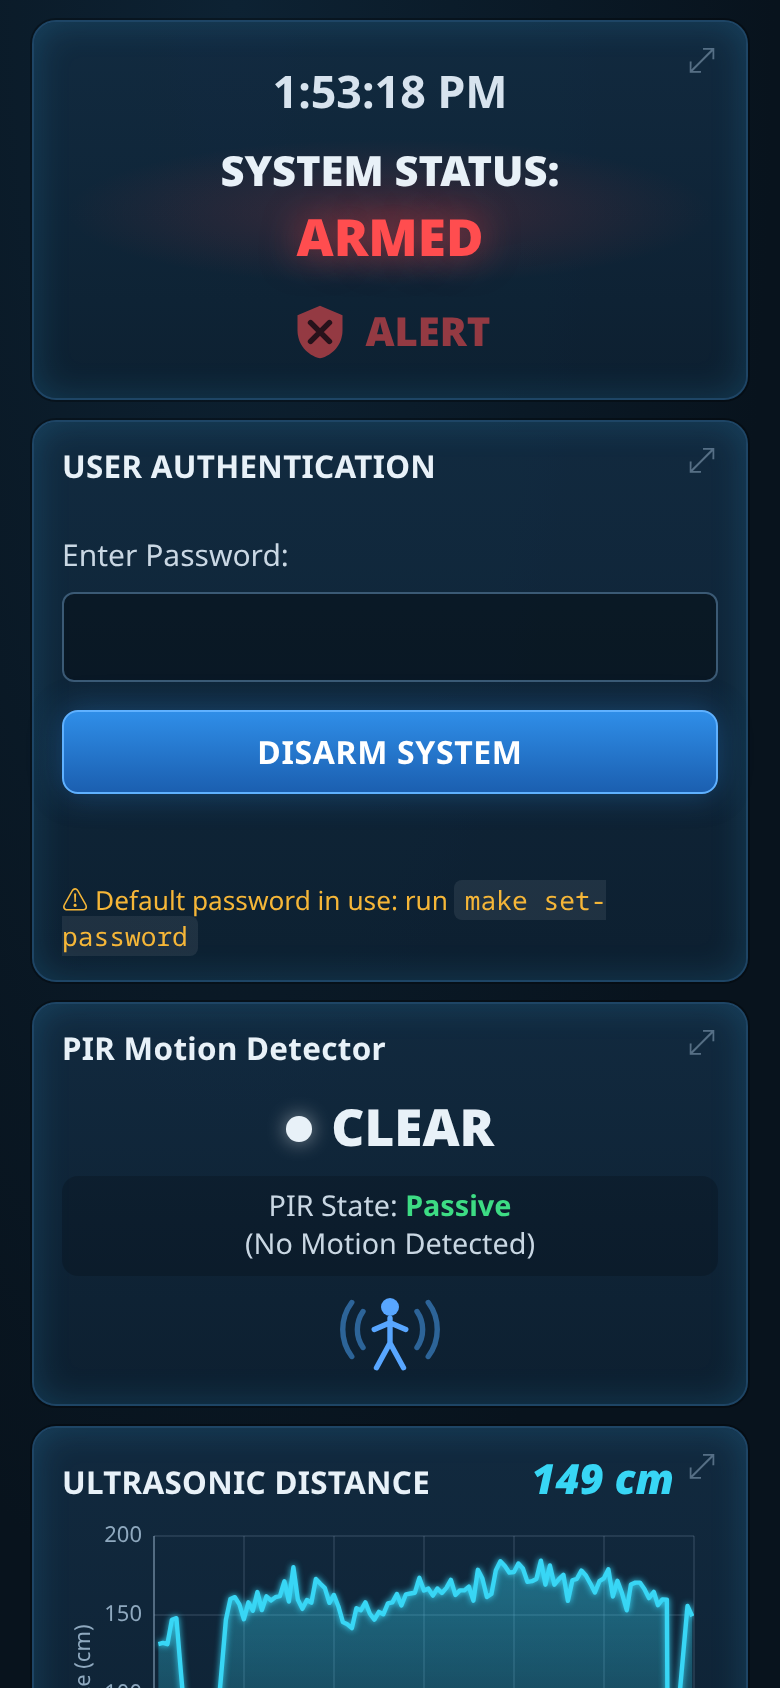
\includegraphics[width=\linewidth]{mobile_4_deconnexion.png}\end{minipage}\hspace{4mm}
\begin{minipage}[c]{0.6\linewidth}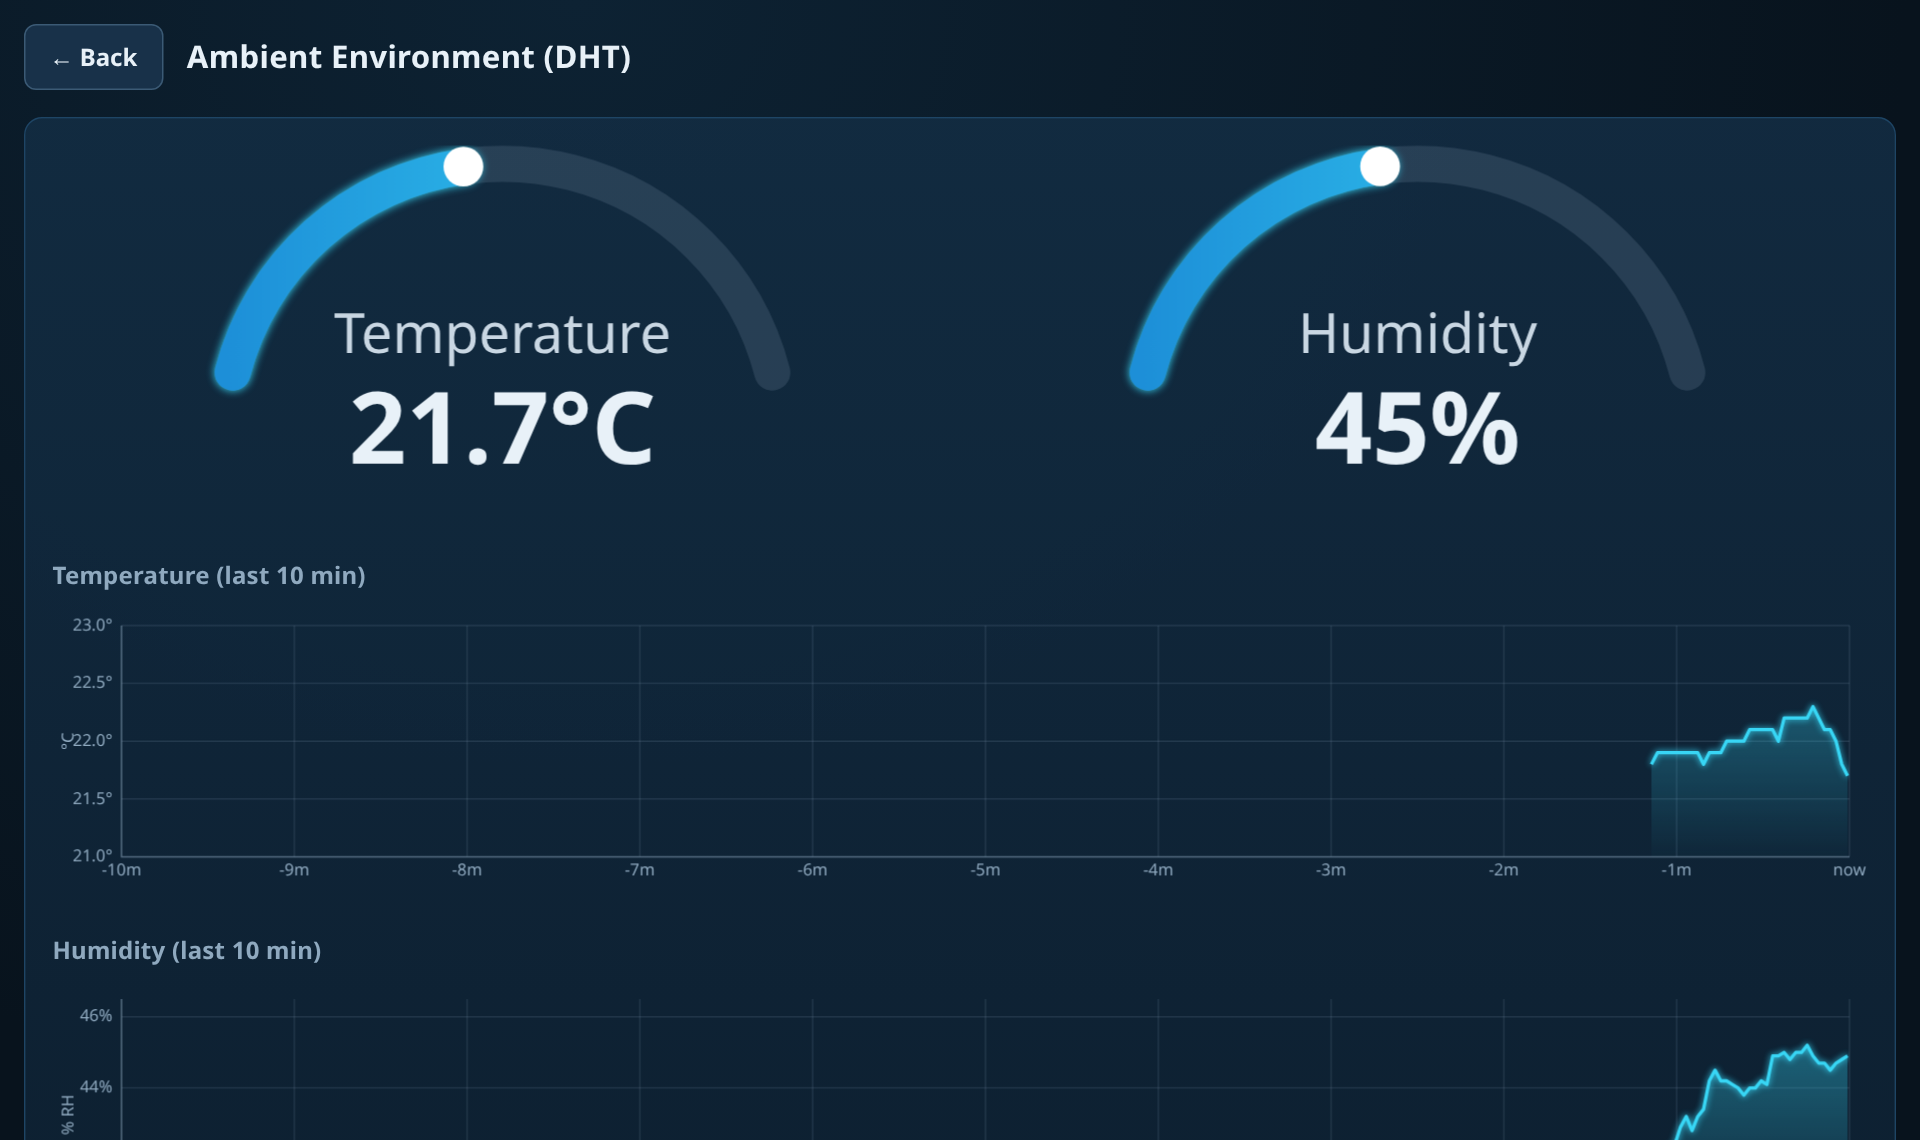
\includegraphics[width=\linewidth]{web_5_vue_agrandie.png}\end{minipage}\\[0.6em]
\small Téléphone (alarme, puis station arrêtée : badge « reconnecting… ») et tuile agrandie.
\end{frame}

% ---------------------------------------------------------------------------
\begin{frame}{Bilan par rapport au cahier des charges}
\small
\begin{columns}[T]
\column{0.32\textwidth}
\textcolor{ok}{\textbf{Fait}}
\begin{itemize}
  \item 3 capteurs, 2 actionneurs
  \item Qt + mode kiosque
  \item Web réactif
  \item Synchro Qt $\leftrightarrow$ web
  \item Actionneurs à distance
  \item Journal SQLite horodaté
\end{itemize}
\column{0.32\textwidth}
\textcolor{partiel}{\textbf{Partiel}}
\begin{itemize}
  \item SSE au lieu de WebSockets
  \item Badge de déconnexion discret
  \item Min/Max/Moy sur 60~s (pas sur 10 relevés en base)
  \item Simulation isolée, mais pas de HAL formelle
\end{itemize}
\column{0.32\textwidth}
\textcolor{non}{\textbf{À faire}}
\begin{itemize}
  \item Écrans Qt Designer (.ui)
  \item Seuils modifiables
  \item Relevé sur demande
  \item Relevés stockés en base
  \item Phase III (matériel)
\end{itemize}
\end{columns}
\end{frame}

% ---------------------------------------------------------------------------
\begin{frame}{Conclusion}
\begin{itemize}
  \item Système complet en simulation : capteurs, alarmes, journal, 2 interfaces synchronisées.
  \item Sécurité prise en compte : mot de passe, empreinte, HTTPS.
  \item 40 tests automatiques.
\end{itemize}
\bigskip
\textbf{Suite :} HAL du sujet, FastAPI + WebSockets, relevés en base, seuils modifiables, puis passage sur la Raspberry Pi.
\end{frame}

\begin{frame}[standout]
Merci !\\[0.5em]
\normalsize Démo en direct et questions
\end{frame}

\end{document}
